%
% $RCSfile: approach.tex,v $
%
% Copyright (C) 2002-2008. Christian Heller.
%
% Permission is granted to copy, distribute and/or modify this document
% under the terms of the GNU Free Documentation License, Version 1.1 or
% any later version published by the Free Software Foundation; with no
% Invariant Sections, with no Front-Cover Texts and with no Back-Cover
% Texts. A copy of the license is included in the section entitled
% "GNU Free Documentation License".
%
% http://www.cybop.net
% - Cybernetics Oriented Programming -
%
% http://www.resmedicinae.org
% - Information in Medicine -
%
% Version: $Revision: 1.1 $ $Date: 2008-08-19 20:41:05 $ $Author: christian $
% Authors: Christian Heller <christian.heller@tuxtax.de>
%

\section{Approach}
\label{approach_heading}

The \emph{Software Gurus} like Gamma, Buschmann, Fowler et al. found their
patterns by \emph{observing} daily software development, architectures, projects
and their standard solutions. This work observes other disciplines of science,
phenomenons of nature, and tries to find parallels to software engineering. It
thus not just wants to provide solutions \emph{using} state-of-the-art techniques
but rather \emph{question} existing techniques and try to find \emph{alternative}
concepts. Because of the steady comparison to principles of nature and other
sciences, this approach is called \emph{cybernetics-oriented}, as explained in
section \ref{cybernetics_heading}.

Although many of the ideas and solutions of this work, in a \emph{bottom-up}
manner, stem from writing source code in practice (following the
\emph{Constructive Development} method of research as announced in section
\ref{method_heading}), the overall approach and explanation of results follow a
\emph{top-down} path. High-level concepts are considered first, before moving
on to an implementation and proof in practice.

%
% $RCSfile: mind_and_brain.tex,v $
%
% Copyright (C) 2002-2008. Christian Heller.
%
% Permission is granted to copy, distribute and/or modify this document
% under the terms of the GNU Free Documentation License, Version 1.1 or
% any later version published by the Free Software Foundation; with no
% Invariant Sections, with no Front-Cover Texts and with no Back-Cover
% Texts. A copy of the license is included in the section entitled
% "GNU Free Documentation License".
%
% http://www.cybop.net
% - Cybernetics Oriented Programming -
%
% http://www.resmedicinae.org
% - Information in Medicine -
%
% Version: $Revision: 1.1 $ $Date: 2008-08-19 20:41:07 $ $Author: christian $
% Authors: Christian Heller <christian.heller@tuxtax.de>
%

\paragraph{Mind and Brain}
\label{mind_and_brain_heading}
\index{Mind and Brain}
\index{Knowledge and System Control}
\index{Software as Passive Knowledge and Active Control}

A first observation, when looking at human beings from a philosophical
perspective, is the separation of \emph{Mind} and \emph{Brain} (Body) (figure
\ref{staticsdynamics_figure}). Accordingly, CYBOP treats computers as
\emph{Systems} owning and processing \emph{Knowledge}. This is not unlike the
idea of \emph{Agent} systems owning a \emph{Knowledge Base} (section
\ref{agent_oriented_programming_heading}). All abstract knowledge that humans
make up belongs to their mind. The brain is merely a physical carrier of
knowledge.

\begin{figure}[ht]
    \begin{center}
        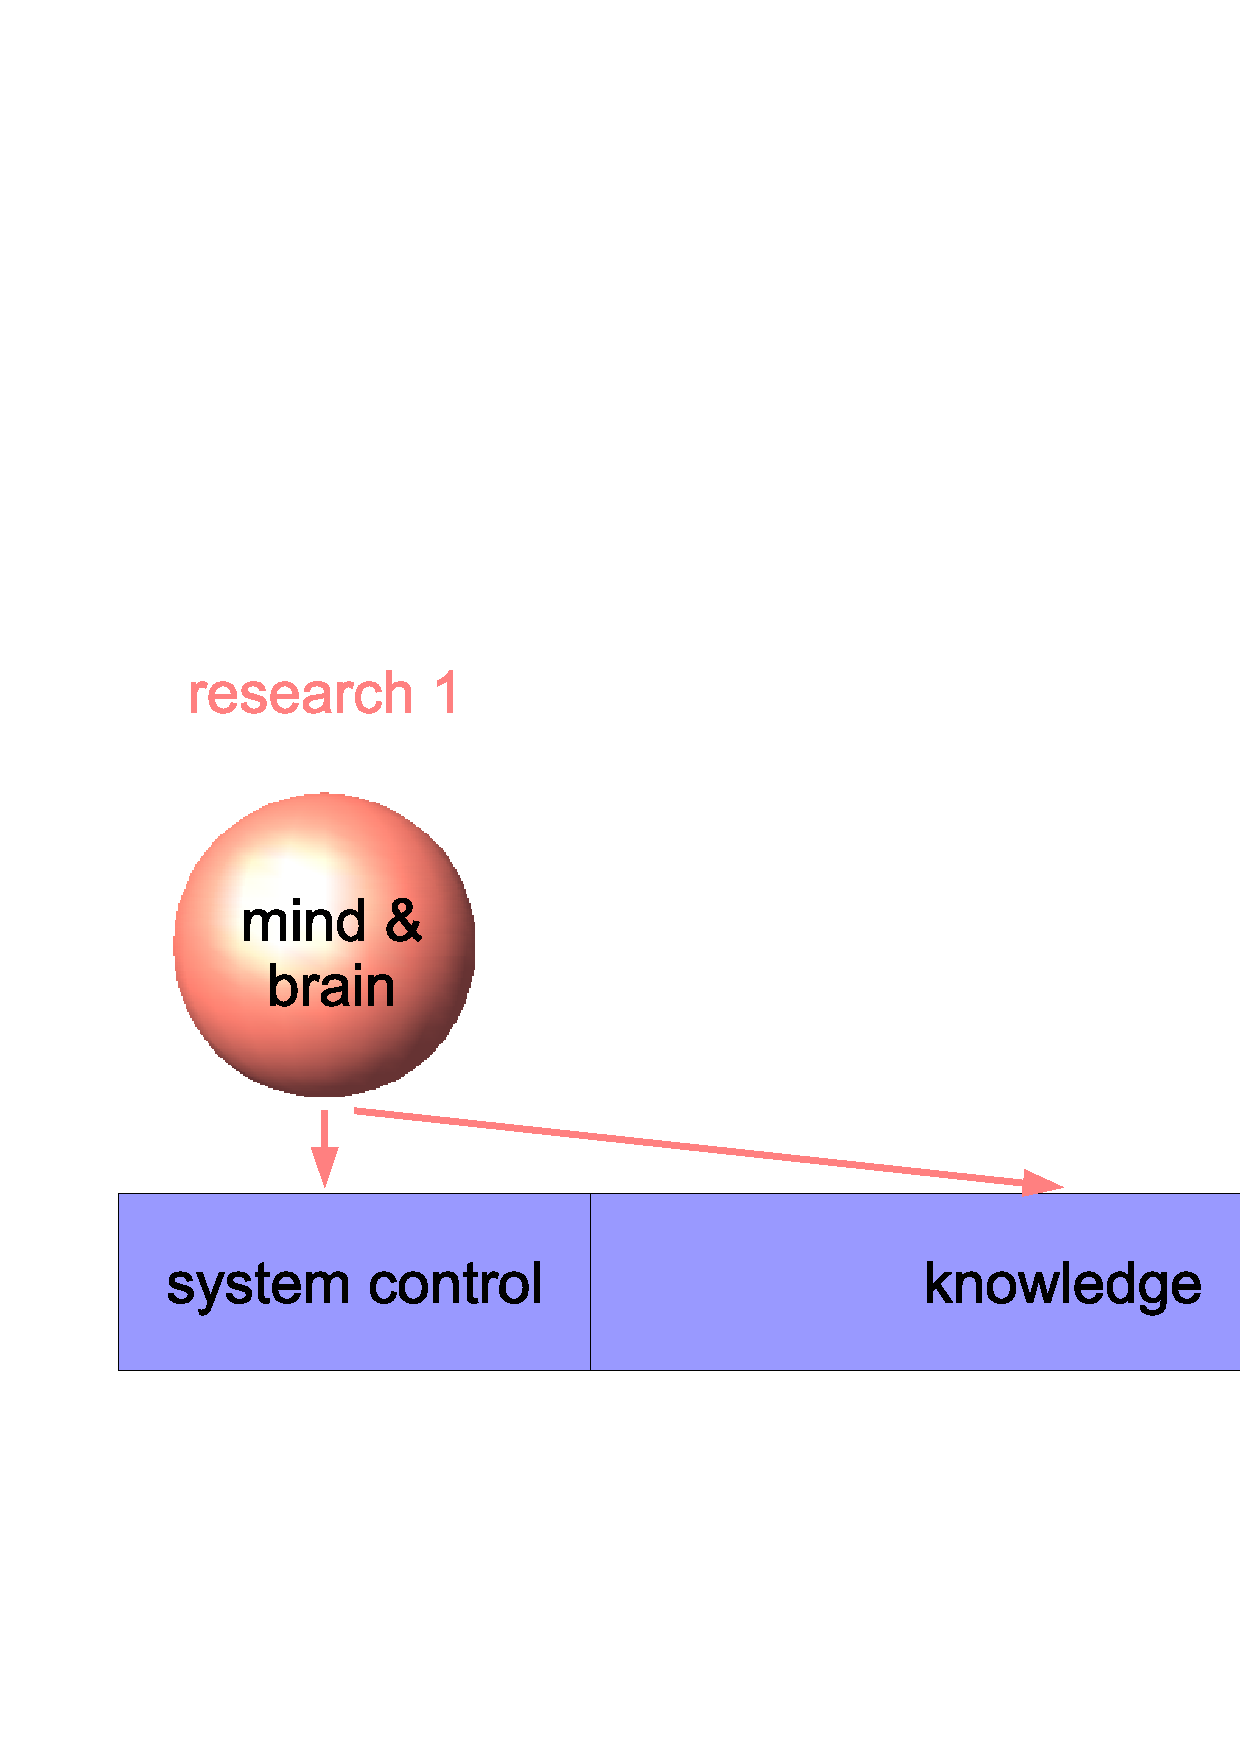
\includegraphics[scale=0.3,angle=-90]{graphic/staticsdynamics.pdf}
        \caption{Separation of Mind/ Brain Leading to Knowledge/ System Control}
        \label{staticsdynamics_figure}
    \end{center}
\end{figure}

Another conclusion resulting from this first observation is that there should
actually be two kinds of software: one representing \emph{passive} knowledge
and the other \emph{actively} controlling a system, close to hardware.

Chapter \ref{statics_and_dynamics_heading} deals with this topic.

%
% $RCSfile: thinking.tex,v $
%
% Copyright (C) 2002-2008. Christian Heller.
%
% Permission is granted to copy, distribute and/or modify this document
% under the terms of the GNU Free Documentation License, Version 1.1 or
% any later version published by the Free Software Foundation; with no
% Invariant Sections, with no Front-Cover Texts and with no Back-Cover
% Texts. A copy of the license is included in the section entitled
% "GNU Free Documentation License".
%
% http://www.cybop.net
% - Cybernetics Oriented Programming -
%
% http://www.resmedicinae.org
% - Information in Medicine -
%
% Version: $Revision: 1.1 $ $Date: 2008-08-19 20:41:09 $ $Author: christian $
% Authors: Christian Heller <christian.heller@tuxtax.de>
%

\paragraph{Human Thinking}
\label{thinking_heading}
\index{Human Thinking}
\index{Discrimination}
\index{Categorisation}
\index{Composition}
\index{Hierarchy}
\index{Hierarchical Knowledge}

Secondly, attention is payed to the concepts of \emph{Human Thinking}, as
investigated by psychology. Many of them are already considered in current
programming languages, for example \emph{Discrimination} and \emph{Categorisation}.
However, an essential one that has not been implemented yet is \emph{Composition}.
Its application would make every abstract model a \emph{Hierarchy} by default.

Hierarchies are not new, they are present in many ways in today's programming.
There are object hierarchies, process hierarchies, design patterns modelling a
hierarchy and more. But: the hierarchy as concept is not \emph{inherent} in the
type system of current programming languages. If it were, then \emph{every}
type would be a \emph{Container} by default.

\begin{figure}[ht]
    \begin{center}
        \includegraphics[scale=0.3,angle=-90]{graphic/hierarchicalknowledge.pdf}
        \caption{Concepts of Human Thinking Leading to Hierarchical Knowledge}
        \label{hierarchicalknowledge_figure}
    \end{center}
\end{figure}

Through the application of these thoughts, the knowledge becomes
\emph{Hierarchical Knowledge} (figure \ref{hierarchicalknowledge_figure}).
Additionally, this work tries to embed knowledge models in an environment of
\emph{Dimensions}, as known from physics, and further properties. Every model
keeps a number of \emph{Meta Information} about its parts. \emph{Positions} in
space or time are one such example.

Chapter \ref{knowledge_schema_heading} further elaborates on these issues.

%
% $RCSfile: data_and_rules.tex,v $
%
% Copyright (C) 2002-2008. Christian Heller.
%
% Permission is granted to copy, distribute and/or modify this document
% under the terms of the GNU Free Documentation License, Version 1.1 or
% any later version published by the Free Software Foundation; with no
% Invariant Sections, with no Front-Cover Texts and with no Back-Cover
% Texts. A copy of the license is included in the section entitled
% "GNU Free Documentation License".
%
% http://www.cybop.net
% - Cybernetics Oriented Programming -
%
% http://www.resmedicinae.org
% - Information in Medicine -
%
% Version: $Revision: 1.1 $ $Date: 2008-08-19 20:41:06 $ $Author: christian $
% Authors: Christian Heller <christian.heller@tuxtax.de>
%

\paragraph{Data and Rules}
\label{data_and_rules_heading}
\index{Data and Rules}
\index{State- and Logic Knowledge}

Thirdly, \emph{State-} and \emph{Logic} knowledge get distinguished (figure
\ref{statelogic_figure}). It is known from neurological research that the human
brain has special communication regions (optical, acoustical, motoric)
responsible for information input and output. Simply spoken, these regions do
nothing else than translating data, that is an input \emph{State} into an
output \emph{State}, according to special rules which can be summarised by the
term \emph{Logic}.

\begin{figure}[ht]
    \begin{center}
        \includegraphics[scale=0.3,angle=-90]{graphic/statelogic.pdf}
        \caption{Translation of Data by Rules Leading to State-/ Logic Knowledge}
        \label{statelogic_figure}
    \end{center}
\end{figure}

This is where systems theory, that uses similar abstractions, comes in. Every
system can be seen as \emph{Black Box} with input/ output (i/o) states and a
translation logic.

When talking about states, this work does \emph{not} mean classical
\emph{State Models} which are often modelled by a \emph{State Chart Diagram}.
A CYBOP state model rather is a composed \emph{Set} of states.

Chapter \ref{state_and_logic_heading} describes more details.

%
% $RCSfile: cybop_approach.tex,v $
%
% Copyright (C) 2002-2008. Christian Heller.
%
% Permission is granted to copy, distribute and/or modify this document
% under the terms of the GNU Free Documentation License, Version 1.1 or
% any later version published by the Free Software Foundation; with no
% Invariant Sections, with no Front-Cover Texts and with no Back-Cover
% Texts. A copy of the license is included in the section entitled
% "GNU Free Documentation License".
%
% http://www.cybop.net
% - Cybernetics Oriented Programming -
%
% http://www.resmedicinae.org
% - Information in Medicine -
%
% Version: $Revision: 1.1 $ $Date: 2008-08-19 20:41:06 $ $Author: christian $
% Authors: Christian Heller <christian.heller@tuxtax.de>
%

\paragraph{CYBOP}
\label{cybop_approach_heading}
\index{Cybernetics Oriented Programming Approach}
\index{CYBOP Approach}
\index{Cybernetics Oriented Language}
\index{CYBOL}
\index{Cybernetics Oriented Interpreter}
\index{CYBOI}
\index{Res Medicinae}

In CYBOP, all knowledge, that is states as well as logic, belongs to the
\emph{Statics} of a system. It is described by fixed structures. The processing
of knowledge at runtime, in order to control a system, is called \emph{Dynamics}.

\begin{figure}[ht]
    \begin{center}
        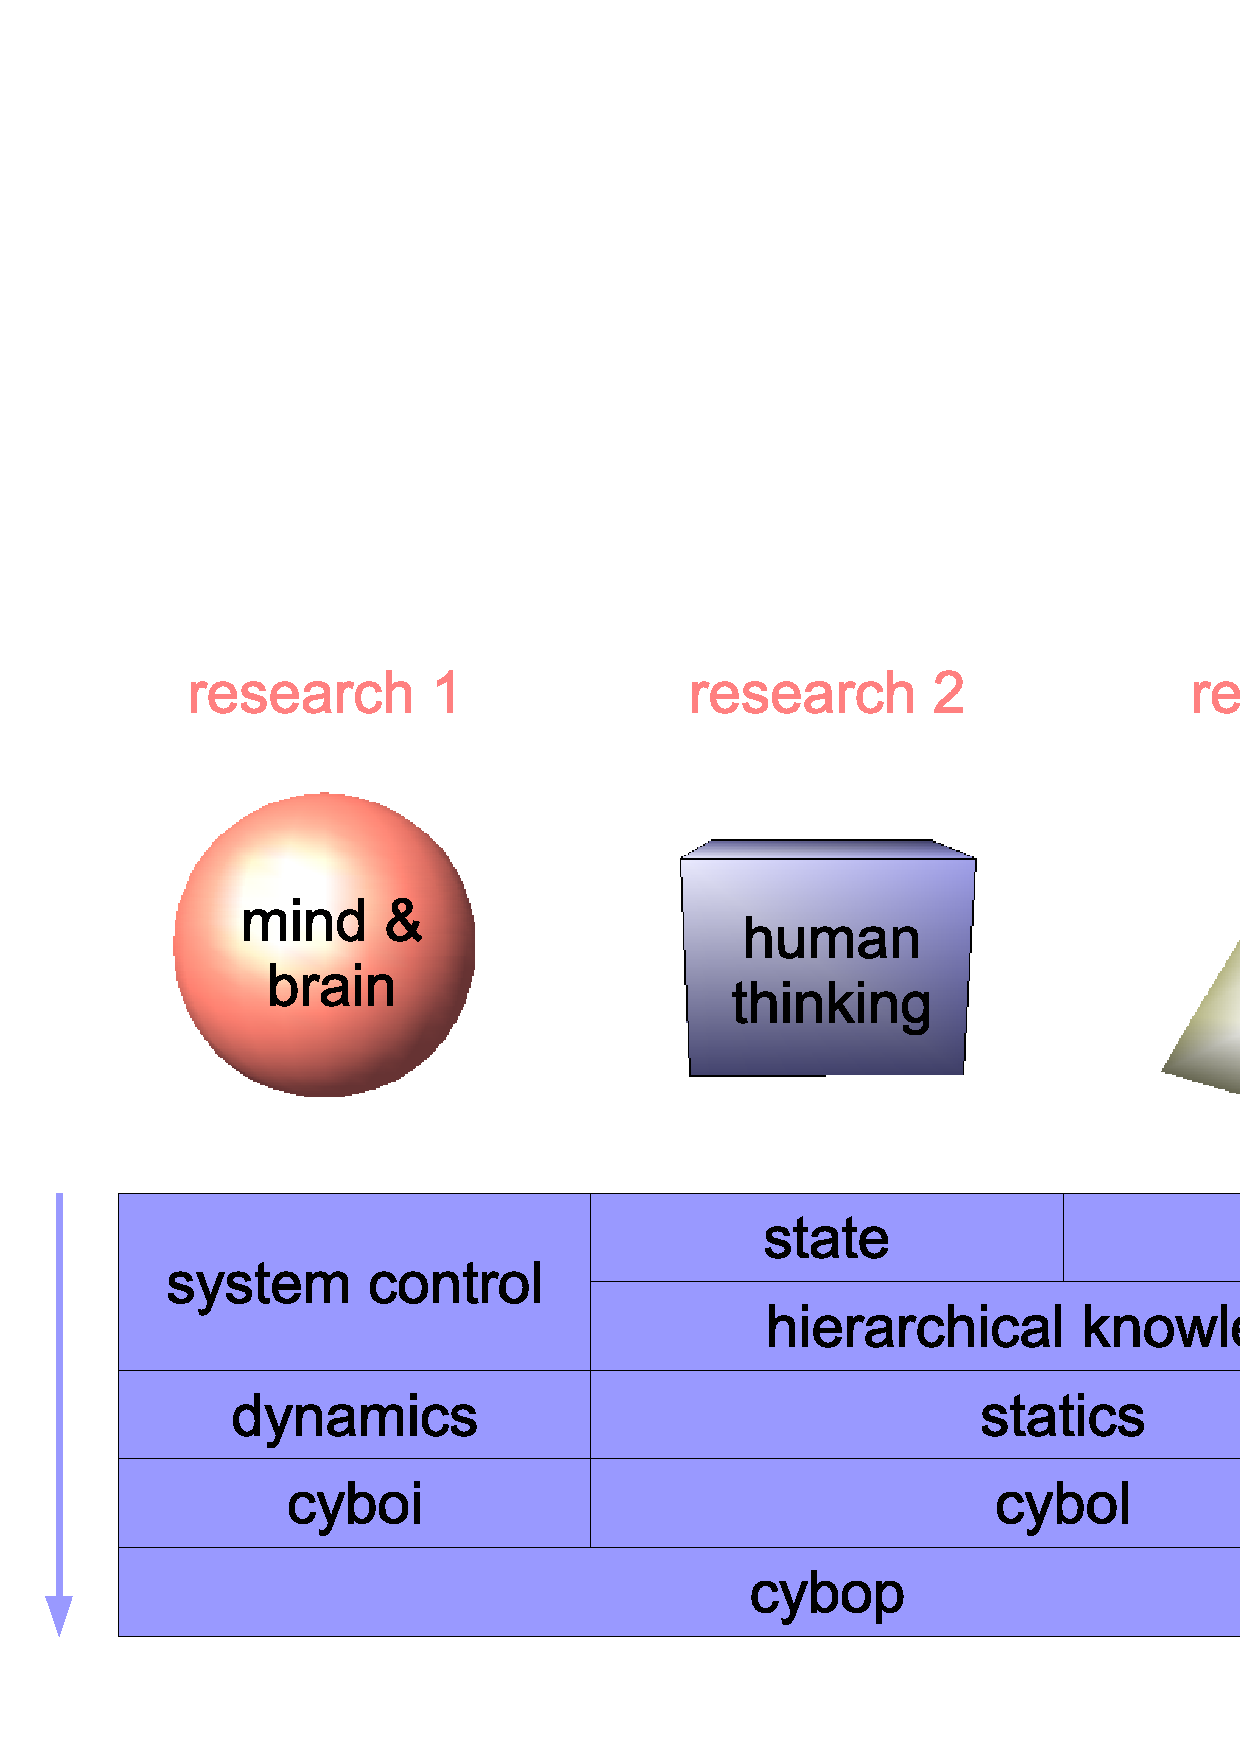
\includegraphics[scale=0.3,angle=-90]{graphic/approach.pdf}
        \caption{Overall CYBOP Approach Based on Statics and Dynamics}
        \label{cybop_approach_figure}
    \end{center}
\end{figure}

The complete modelling and storage of static knowledge requires a formal
language, which gets introduced as \emph{Cybernetics Oriented Language} (CYBOL)
in this work. Its dynamic processing, close to hardware, is guaranteed by the
\emph{Cybernetics Oriented Interpreter} (CYBOI) which is needed to run systems
defined in CYBOL (figure \ref{cybop_approach_figure}).

Chapters \ref{cybernetics_oriented_language_heading} and
\ref{cybernetics_oriented_interpreter_heading} explain CYBOL and CYBOI,
respectively. Both are used in the \emph{Res Medicinae} prototype application
which gets introduced in chapter \ref{res_medicinae_heading}. Altogether,
CYBOL, CYBOI and the theoretical concepts behind are called
\emph{Cybernetics Oriented Programming} (CYBOP).

